\section{ปัญหาแบบอิลล์โพสและวิธีการเร็กกิวลาร์ไลซ์เซชัน}

\begin{Definition}
    (ปัญหาแบบเวลล์โพส) เราจะเรียกปัญหาที่กำหนดว่าเป็นปัญหาแบบเวลล์โพส เมื่อเงื่อนไขทุกข้อต่อไปนี้เป็นจริง
    \begin{enumerate}
        \item ปัญหามีคำตอบ
        \item ปัญหามีเพียงคำตอบเพียงหนึ่งเดียว
        \item คำตอบของปัญหาขึ้นอยู่กับความต่อเนื่องของข้อมูล
    \end{enumerate}    
    หากข้อใดข้อหนึ่งไม่จริง จะเรียกปัญหาที่กำหนดว่า ปัญหาอิลล์โพส
\end{Definition}


\begin{Example}
    ปัญหาการหาค่า $x$ และ $y$ ที่ทำให้ $x+y = 5$ เป็นปัญหาที่มีหลายคำตอบ ดังนั้นปัญหานี้เป็นปัญหาแบบอิลล์โพส
    \label{example:x_plus_y_5}
\end{Example}

\hspace{1cm} ปัญหาการต่อเติมภาพเป็นปัญหาแบบอิลล์โพสเนื่องจากคำตอบในบริเวณโดเมนต่อเติมไม่ได้มีเพียงคำตอบเดียว ตัวอย่างเช่น รูปที่ \ref{image:meme_elephant} ภาพช้างทีเสียหาย\footnote{ภาพจาก https://9gag.com/gag/aer4VwB สืบค้นเมื่อ 10 มีนาคม 2562} ในบริเวณส่วนสีแดงซึ่งภาพเกิดความเสียหายขึ้น อาจจะมีคำตอบเป็นขาของช้าง หรือมีคำตอบเป็นสิงโตดังในภาพก็ได้

\begin{figure}[H]
    \centering
    \begin{subfigure}[b]{0.48\textwidth}
        
\includegraphics[width=0.85\linewidth]{image/meme_elephant.png}
    \end{subfigure}
    \begin{subfigure}[b]{0.48\textwidth}
        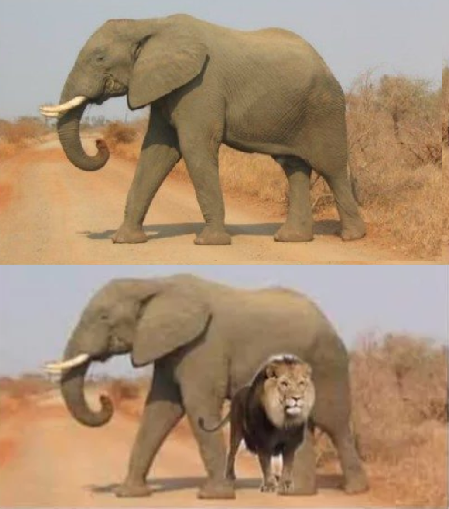
\includegraphics[width=0.85\linewidth]{image/meme_elephant_answer.png}
    \end{subfigure}
    \caption[a]{(ซ้าย) ปัญหาการต่อเติมภาพ (ขวา) ตัวอย่างคำตอบที่เป็นไปได้}
    \label{image:meme_elephant}
\end{figure}


\subsection{วิธีการเร็กกิวลาร์ไรซ์เซชัน}
\hspace{1cm} วิธีเร็กกิวลาร์ไรซ์เซชัน (Regularization) เป็นวิธีการทางคณิตศาสตร์ที่นิยมอย่างแพร่หลายในการแก้ปัญหาแบบอิลล์โพสคิดค้นโดย Tikhonov \cite{ref:regularization} 

\hspace{1cm} โดยวิธีการนี้จะทำการแก้ปัญหาแบบอิลล์โพสโดยการเพิ่มเงื่อนไขเข้าไปในปัญหาเพื่อให้คำตอบที่ได้เป็นเซตคำตอบที่อยู่ในเซตของคำตอบที่เป็นไปได้ 

\begin{Example}
    กำหนดให้ x + y = 5 จงหา x และ y ที่ทำให้สมการเป็นจริง
    จะพบว่าปัญหานี้เป็นปัญหาแบบอิลล์โพสเนื่องจากมีคำตอบได้หลายคำตอบ \\
    \hspace{1cm} หลังจากใช้แนวคิดของเร็กกิวลาร์ไรซ์เซชันโดยการเพิ่มเงื่อนไขว่า $\sqrt{x^2+y^2}$ มีค่าน้อยที่สุด
    จึงได้ว่า  $x = 2.5$ และ $y = 2.5$ เป็นคำตอบของปัญหาที่สอดคล้องกับเงื่อนไขทางคณิตศาสตร์ที่ต้องการ
\end{Example}